\documentclass{beamer}
\beamertemplatenavigationsymbolsempty
\setbeamertemplate{footline}[frame number]
\setbeamertemplate{bibliography item}{\insertbiblabel}
\setbeamertemplate{caption}[numbered]
\usepackage{graphicx}
	\graphicspath{{images/}} 
\usepackage{cite}
\usepackage{courier}
\usepackage{hyperref}
    \hypersetup{colorlinks=true,allcolors=blue}
\usepackage{listings}
	\lstset{
  		basicstyle=\ttfamily,
  		frame=none,
  		breaklines=true,
  		numbers=left,
  		xleftmargin=2em,
  		framexleftmargin=0em,
    	emphstyle=\textbf,
    	float=t
	}
	\lstdefinestyle{ocl}{
  		emph={
        	context, inv
    	}
	}
	\lstdefinestyle{cbp}{
	    basicstyle=\ttfamily\scriptsize,
  		emph={
        	session, create, of, type,
        	set, to, add, hire
    	}
	}
	\lstdefinestyle{xmi}{
		basicstyle=\ttfamily\scriptsize,
  		emph={
        	Employee, manages
    	}
	}
	\lstdefinestyle{xml}{
	    basicstyle=\ttfamily\tiny,
  		emph={
        	register, create, add, to, resource,
        	from, eattribute, remove, ereference,
        	set, unset, session, Roy, Jen,
        	Moss, Richmond
    	}
	}
	\lstdefinestyle{java}{
	    basicstyle=\ttfamily\tiny,
  		emph={
        	case, UNSET,
        	instanceof, else, if, void,
        	new, UnsetEAttributeEvent,
        	UnsetEReferenceEvent,
        	@override, public, class, extends
    	}
	}



\begin{document}

    \title[Crisis] % 
{Turning Models Inside Out}
%\subtitle{Evidence from India}
\author[Author, Anders] % (optional, for multiple authors)
{Alfa Yohannis\and Fiona Polack \and Dimitris Kolovos}
\institute[University of York] % (optional)
{
  Department of Computer Science\\
University of York\\
York, United Kingdom\\
\{ary506, fiona.polack, dimitris.kolovos\}@york.ac.uk
}
\date[18 September 2017]
{FlexMDE @ MODELS'17}
%\\18 September 2017\\Austin, Texas, USA
\subject{Computer Science}

\frame{\titlepage}

\begin{frame}
\frametitle{Introduction}
\begin{itemize}
    \item Model-based software engineering in the context of large and complex systems demands ability to process large models.
    \item One way to tackle this is through the use of incremental model processing techniques.
    \item Current incremental model processing techniques only deliver limited performance benefit due to:
    \begin{itemize}
        \item Slow inprecise model change detection capabilities, and
        \item Limited to a single-developer environment -- not realistic for software development projects.
    \end{itemize}    
\end{itemize}
\end{frame}
  
\begin{frame}
\frametitle{Our Aim}
\begin{itemize}
\item We aims at enabling flexible and high-performance incremental model processing through change-based model persistence.
\item Instead of persisting snapshots of the state of models, we propose turning models inside out and persisting their change history.
\item It has the potential to deliver step-change performance benefits in incremental model processing, as well as a wide range of other benefits and novel capabilities.
\end{itemize}  
\end{frame}

\begin{frame}
\frametitle{An Example of Change-based Techniques (1)}
\label{sec:An example_of_change-based_techniques_1}
\framesubtitle{Report Generation Optimisation of an Organisational Chart Model}
\begin{figure}[ht]
\centering
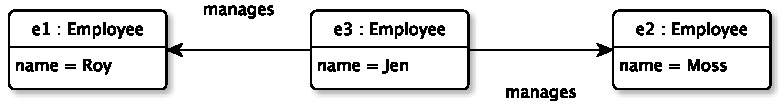
\includegraphics[width=\linewidth]{initial_chart}
\caption{Initial version of the organisational chart model.}
\label{fig:initial_chart}
\end{figure}

\begin{figure}[ht]
\centering
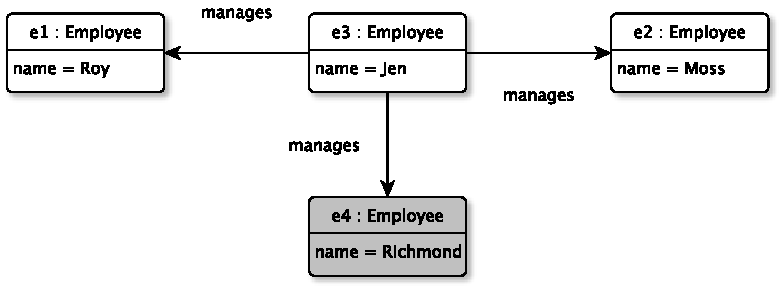
\includegraphics[width=\linewidth]{modified_chart}
\caption{Modified version of the organisational chart model of Fig. \ref{fig:initial_chart}.}
\label{fig:modified_chart}
\end{figure}
\end{frame}


\begin{frame}
\frametitle{An Example of Change-based Techniques (2)}
\label{sec:An example_of_change-based_techniques_2}
\framesubtitle{Report Generation Optimisation of an Organisational Chart Model}
\begin{itemize}
\item We have two consecutive organisational chart models (Fig. \ref{fig:initial_chart} and \ref{fig:modified_chart}), which after every modification, they need to be:
\begin{itemize}
\item Validated against a domain-specific constraint (that no employee directly manages more than 7 other employees).
\item Transformed into a number of employee reports through a model-to-text transformation. Each report contains the name of the employee, and the names of her direct subordinates.
\end{itemize}
\item At the end of Fig. \ref{fig:initial_chart}'s modification:
\begin{itemize}
\item All employees satisfy the constrain (Roy, Jen, Moss).
\item Three reports are generated (Roy, Jen, Moss).
\end{itemize}
\item At the end of Fig. \ref{fig:modified_chart}'s modification:
    \begin{itemize}
    \item All employees satisfy the constrain (Roy, Jen, Moss, Richmond).
    \item Two reports are (re)generated (Jen, Richmond).
\end{itemize}
\end{itemize}
\end{frame}

\begin{frame}
\frametitle{An Example of Change-based Techniques (3)}
\label{sec:An example_of_change-based_techniques_3}
\framesubtitle{Report Generation Optimisation of an Organisational Chart Model}
Non-incremental vs incremental approaches on optimising model validation and transformation.
\begin{itemize}
\item Non-incremental approach:
    \begin{itemize}
    \item (re)evaluates the constrain against all the employees
    \item (re)generates reports for all the employees
    \end{itemize}
\item Incremental approach:
    \begin{itemize}
    \item  only (re)evaluates the constrain against Jen and Richmond
    \item only (re)generates reports for Jen and Richmond
    \end{itemize}
\end{itemize}
Non-incremental execution can become a significant bottleneck for large evolving models, particularly in the latter phases of the development cycle when many small changes made to fine-tune the system\cite{selic2003pragmatics}.
\end{frame}

\begin{frame}
\frametitle{Requirements for Incremental Engine}
As demonstrated by Egyed \cite{egyed2011automatically}, to achieve incremental re-execution of (deterministic) queries on structured models, an execution engine needs to:
\begin{enumerate}
\item Record model element property accesses during the initial execution of the queries;
\item Identify new and deleted elements and modified model element properties in the new version of the model;
\item Combine the information collected in the steps above to identify the subset of (potentially) affected rules/queries/templates that need to be re-executed.
\end{enumerate}
\end{frame}

\begin{frame}
\frametitle{ Identifying Changes in Models}
Two approaches for identifying changes in models to enable incremental model processing.
\begin{itemize}
\item \textbf{Notifications}. The engine listens to the notification facility of a modelling tool and receives notifications as soon as the model is modified (add a new employee). 
\begin{itemize}
\item Applied by: IncQuery incremental pattern matching framework \cite{rath2012derived}, ReactiveATL incremental model-to-model transformation engine \cite{ogunyomi2015property}. 
\item Advantages: fine-grained change notification facilities are provided for free by modelling tools.
\item Drawbacks: poor for collaborative development when a model is modified by different developers.
\end{itemize} 
\item \textbf{Model Differencing}. A Model is compared to its previous version and the engine computes their differences.    
\begin{itemize}
\item Applied by: SiDiff \cite{kelter2005generic} or EMFCompare\footnote{\url{https://www.eclipse.org/emf/compare/}}).
\item Advantages: works well in a collaborative
development with different roles and responsibility of developers.
\item Drawbacks: computationally expensive, memory-greedy.
\end{itemize}
\end{itemize}
\end{frame}

\begin{frame}[fragile]
\frametitle{A State-Based Representation}
A state-based representation of the model of Fig. \ref{fig:modified_chart} in XMI.
\begin{lstlisting}[style=xmi,label=lst:xmimodel]
<Employee xmi:id="e2" name="Jen">
  <manages xmi:id="e1" name="Roy"/>
  <manages xmi:id="e3" name="Moss"/>
  <manages xmi:id="e4" name="Richmond"/>
</Employee>
\end{lstlisting}
\end{frame}

\begin{frame}[fragile]
\frametitle{A Change-based Persistence Representation}
A change-based representation of the model of Fig. \ref{fig:modified_chart}.
\begin{lstlisting}[style=xml,label=lst:cbpmodel]
<session id="s1"/>
<create eclass="Employee" epackage="employee" id="0"/>
<add-to-resource position="0"><value eobject="0"/></add-to-resource>
<set-eattribute name="name" target="0"><value literal="Roy"/></set-eattribute>
<create eclass="Employee" epackage="employee" id="1"/>
<add-to-resource position="1"><value eobject="1"/></add-to-resource>
<set-eattribute name="name" target="1"><value literal="Jen"/></set-eattribute>
<create eclass="Employee" epackage="employee" id="2"/>
<add-to-resource position="2"><value eobject="2"/></add-to-resource>
<set-eattribute name="name" target="1"><value literal="Moss"/></set-eattribute>
<remove-from-resource><value eobject="0"/></remove-from-resource>
<add-to-ereference name="manages" position="0" target="1"><value eobject="0"/></add-to-ereference>
<remove-from-resource><value eobject="2"/></remove-from-resource>
<add-to-ereference name="manages" position="1" target="1"><value eobject="2"/></add-to-ereference>
<session id="s2"/>
<create eclass="Employee" epackage="employee" id="3"/>
<add-to-resource position="1"><value eobject="3"/></add-to-resource>
<set-eattribute name="name" target="3"><value literal="Richmond"/></set-eattribute>
<remove-from-resource><value eobject="3"/></remove-from-resource>
<add-to-ereference name="manages" position="2" target="2"><value eobject="3"/></add-to-ereference>
\end{lstlisting}
\end{frame}

\begin{frame}
\frametitle{Prototype Implementation}
\begin{itemize}
\item We have implemented a prototype. The prototype is available under \url{https://github.com/epsilonlabs/emf-cbp}.
\item The change-based model persistence format uses the notification facilities provided by the Eclipse Modelling Framework. 
\begin{itemize}
\item \emph{EContentAdapter} class  {\tiny \url{http://download.eclipse.org/modeling/emf/emf/javadoc/2.11/org/eclipse/emf/ecore/util/EContentAdapter.html}} 
\item \emph{Notification} class {\tiny\url{http://download.eclipse.org/modeling/emf/emf/javadoc/2.11/org/eclipse/emf/common/notify/Notification.html}}
\end{itemize}
\item Basically, it works by capturing events from the \emph{Notification}: filtering and putting the events into a change-event list, and persisting them into a change-based representation.
\end{itemize}
\end{frame}

\begin{frame}
\frametitle{Event Classes to Represent Changes of Models}
\begin{figure}[htbh]
\centering
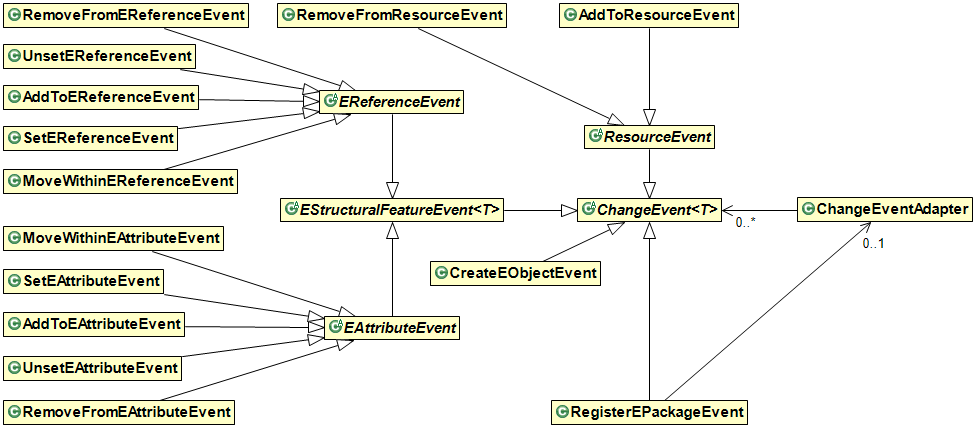
\includegraphics[width=\linewidth]{events}
\caption{Event classes to represent changes of models.}
\label{fig:events}
\end{figure}
\end{frame}

\begin{frame}[fragile]
\frametitle{Java Code to Handle Notifications}
Simplified Java code to handle notification events.
\begin{lstlisting}[style=java,label=lst:javacode]
public class ChangeEventAdapter extends EContentAdapter {
...
@override
public void notifyChanged(Notification n) {
  ...
  switch (n.getEventType()) {
    ... // other events
    case Notification.UNSET: {
    if (n.getNotifier() instanceof EObject) {
      EStructuralFeature feature = (EStructuralFeature) n.getFeature();
        if (feature instanceof EAttribute) {
            event = new UnsetEAttributeEvent();
          } else if (feature instanceof EReference) {
            event = new UnsetEReferenceEvent();
          }
      } break;
    } 
    ... // other events
\end{lstlisting}

\end{frame}

\begin{frame}[fragile]
\frametitle{Factory, resources, and ChangeEventAdapter classes}
\begin{figure}[th]
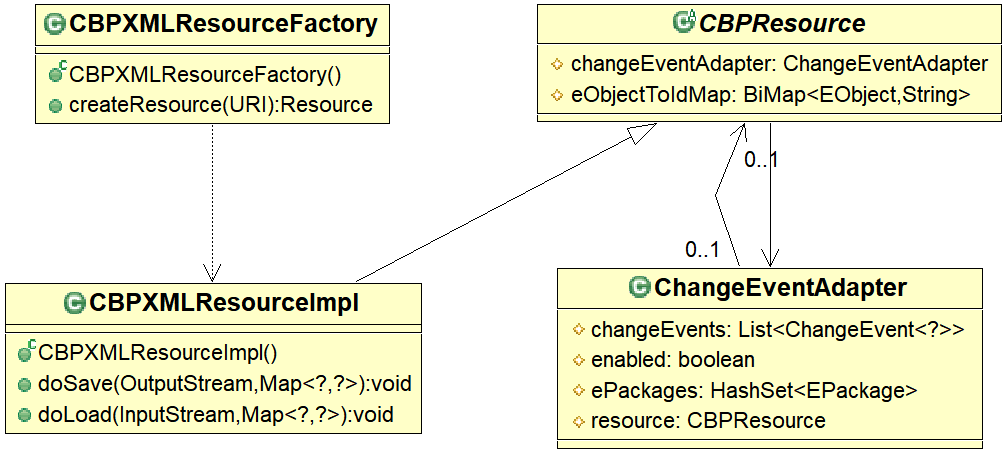
\includegraphics[scale=0.4]{resources}
\caption{Factory, resources, and ChangeEventAdapter classes.}
\end{figure}
\end{frame}


\begin{frame}
\frametitle{Benefits and Novel Capabilities}
\begin{itemize}
\item \textbf{Tool Support}. With appropriate tool support, modellers will be able to ``replay" the change history of a model (e.g. to understand design decisions made by other developers). 
\item \textbf{Analytics}. By analysing models serialised in the proposed representation, modelling tool vendors will be able to develop insights into how modellers actually use their tools in practice.
\item \textbf{Tracing}. By attaching additional information to each session, we can trace back the developer that made changes, or the requirements/bug reports that triggered them.
\item \textbf{Performance}. Persisting changes to large models after an editing session will be significantly faster, as well as the performance and precision of model comparison and merging can be substantially improved.
\end{itemize}
\end{frame}

\begin{frame}
\frametitle{Challenges and Future Work}
\begin{itemize}
\item \textbf{Loading Overhead}. Loading models into memory by naively replaying the entire change history has a significant overhead. To address it, we will develop dedicated algorithms and data structures that will reduce the cost of the loading (e.g. ignoring events that are later overridden or cancelled out by other events). 

\item \textbf{Fast-Growing Model Files}. A file for persisting models in a change-based format will grow in size faster than their state-based counterparts. To address this challenge, we will (1) propose sound change-compression operations (e.g. remove older/unused information) to reduce size; (2) develop a compact textual format to minimise space required (a textual line-separated format is desirable for compatibility with file-based version control systems); (3) propose a hybrid model persistence format to incorporate change-based and state-based information. 
\end{itemize}
\end{frame}


\begin{frame}
\frametitle{Evaluations}
\begin{itemize}
\item \textbf{Vs Existing Algorithms/Tools}. Evaluation where there are existing approaches that the algorithms and tools developed in this research seek to outperform (e.g. change-based incremental validation vs. state-based incremental validation), comparative evaluation will be conducted to assess the benefits and limitations of our approaches. 
\item \textbf{Vs Seek-to-be-improved Baselines}. For algorithms and tools that have no direct competitors in the literature, their contributions will be assessed in comparison to the baseline they seek to improve (e.g. vs persisting full change histories).
\end{itemize}
\end{frame}

\begin{frame}
\frametitle{Conclusions}
\begin{itemize}
\item This research aims at enabling high-performance incremental model processing in collaborative development settings through turning models inside out and persisting their change history.
\item A prototype implementation of a change-based persistence format has been presented, the main envisioned challenges have been listed and an evaluation strategy has been outlined.
\item The proposed approach also has the potential to enable model analytics, more fine-grained tracing and to improve the precision and performance of model comparison and merging. 
\end{itemize}
\end{frame}

\begin{frame}
\frametitle{References}
\scriptsize
\bibliographystyle{IEEEtran}
\bibliography{references}
\end{frame}

\end{document}